\documentclass[11pt, a4paper]{scrartcl}

% Encodage et langue
\usepackage[utf8]{inputenc}
\usepackage[T1]{fontenc}
\usepackage[french]{babel}

% Mise en page et graphismes
\usepackage[margin=2.5cm]{geometry}
\usepackage{graphicx}
\usepackage{tabularx}
\usepackage{hyperref}
\usepackage{scrlayer-scrpage}
\usepackage{float}
\usepackage{xcolor}
\usepackage{tcolorbox}
\usepackage{placeins}

\DeclareUnicodeCharacter{251C}{\mbox{|}}
\DeclareUnicodeCharacter{2500}{\mbox{-}}
\DeclareUnicodeCharacter{2514}{\mbox{`}}
\DeclareUnicodeCharacter{2502}{\mbox{|}}

% Variables globales pour la page de garde
\def\VARcompany{Application Web - L3 MIAGE}
\def\VARtitle{Rapport de Conception Logicielle}
\def\VARdate{\today}

\begin{document}
	\shorthandoff{:}
	
	% Inclusion de la page de garde (cover.tex)
	\input{cover.tex}
	
	\newpage
	
	\pagenumbering{arabic} % Réactive la numérotation normale
	\setcounter{page}{1}   % Force cette page à être la page 1
	\cfoot{}
	\ofoot{Page \thepage}  % Place "Page X" en bas à droite (Outer FOOT)
	
	% Inclusion des chapitres
	\section{Introduction}

Ce rapport documente la conception architecturale et technique de notre projet de fin de semestre pour l'UE Application Web. Notre objectif principal était de concevoir et de développer une suite de trois jeux web distincts, exploitant chacun une technologie de rendu différente. Nous avons ainsi implémenté un jeu basé sur la manipulation dynamique du DOM, un jeu d'artillerie exploitant le Canvas HTML5 en deux dimensions, et enfin un jeu hybride en trois dimensions utilisant le moteur BabylonJS couplé à WebAssembly. L'ensemble de cet écosystème client est unifié par une architecture serveur commune développée en Node.js, chargée de gérer l'authentification des joueurs et la centralisation des scores.

Plutôt que d'adopter une approche de développement empirique au fil de l'eau, nous avons fait le choix de structurer notre code autour de principes d'ingénierie logicielle stricts. Pour nous assister dans cette démarche complexe, nous avons fait appel à des modèles d'intelligence artificielle générative. Nos spécifications à l'attention de l'IA n'ont délibérément pas été formulées comme de simples requêtes de génération de code brut, mais comme des contraintes architecturales. Nous avons rédigé des invites détaillant avec précision les contrats d'interface attendus, les patrons de conception à implémenter et les hiérarchies d'héritage à respecter de manière absolue. Cette méthode de spécification par l'architecture a forcé l'assistant IA à produire des modules hautement découplés et réutilisables plutôt que du code monolithique, garantissant ainsi une base de travail évolutive et propice au travail collaboratif.
	\newpage
	\section{Conception du Jeu Canvas}

Le jeu développé sur le Canvas HTML5 représente le rigeur de notre réflexion architecturale, se distinguant par une modularité exemplaire et une application forte des concepts de la programmation orientée objet. Afin de garantir des performances optimales et une grande facilité de maintenance, nous avons strictement séparé le moteur de jeu, la gestion de l'interface utilisateur, les calculs physiques et la logique métier. 

Le cœur du système est orchestré par une classe principale agissant comme un point d'entrée, qui délègue ensuite les responsabilités temporelles et spatiales à des gestionnaires spécialisés. Un gestionnaire de niveau s'occupe de l'instanciation des cartes et du placement des entités à partir de fichiers de configuration externes, tandis qu'un gestionnaire de tours régule le flux du combat et évalue en continu les conditions de victoire ou de défaite. En parallèle, un gestionnaire d'interface fait le pont entre les nécessités de rendu graphique sur le Canvas et les superpositions d'éléments HTML du DOM pour les menus et les barres d'outils.

% ==========================================
% INSERTION DU DIAGRAMME 1 : CORE ENGINE
% Ce diagramme illustre les relations entre Game, UIManager, LevelManager, etc.
% ==========================================
\FloatBarrier
\begin{figure}[H]
	\centering
	% Remplacez 'core_engine.png' par le nom exact de votre image exportée
	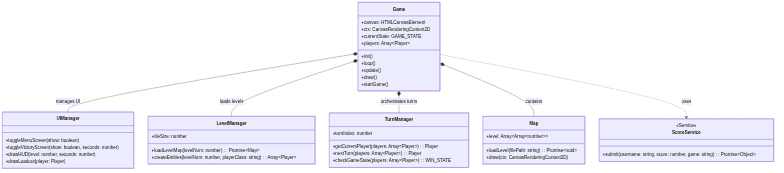
\includegraphics[width=1\textwidth]{canvas_1.png}
	\caption{Architecture du moteur principal et de ses gestionnaires}
	\label{fig:core_engine}
\end{figure}
\FloatBarrier

La hiérarchie des entités a été pensée pour maximiser la factorisation du code tout en permettant une grande diversité de comportements à l'écran. Toutes les entités physiques, qu'elles soient contrôlées par un joueur humain ou par l'ordinateur, héritent d'une classe de base abstraite définissant la physique spatiale, les règles de collisions environnementales et la gestion des points de vie. À partir de cette fondation solide, nous avons dérivé des classes spécifiques pour les joueurs humains, telles que l'archer ou le mage, ainsi que des classes distinctes pour les adversaires, comme les gobelins ou le dragon. Cette séparation claire des responsabilités structurelles permet d'ajouter de nouvelles classes de personnages de manière triviale, simplement en instanciant une nouvelle classe fille et en lui attribuant des statistiques ou des dimensions propres, sans risquer de perturber la physique fondamentale du jeu.

% ==========================================
% INSERTION DU DIAGRAMME 2 : HIÉRARCHIE DES ENTITÉS
% Ce diagramme montre l'héritage de GraphicalObject -> Player -> Bot / Archer / Mage, etc.
% ==========================================
\FloatBarrier
\begin{figure}[H]
	\centering
	% Remplacez 'entities.png' par le nom exact de votre image exportée
	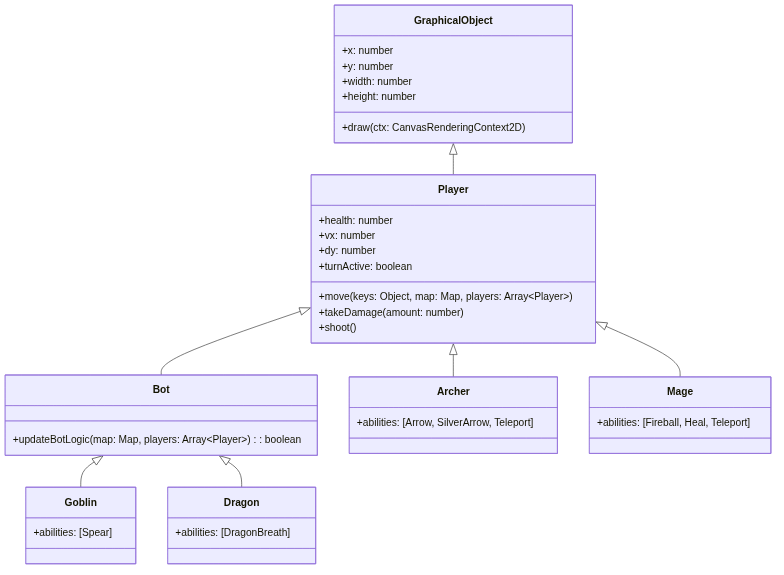
\includegraphics[width=1\textwidth]{canvas_2.png}
	\caption{Hiérarchie d'héritage des entités physiques (Joueurs et IA)}
	\label{fig:entities}
\end{figure}
\FloatBarrier

Le système d'armement et de projectiles suit une philosophie d'héritage similaire, garantissant une gestion unifiée de la balistique. Un objet projectile de base implémente les algorithmes de détection de collision et de cinématique linéaire dans un espace assujetti à la gravité. Des projectiles plus complexes viennent ensuite surcharger ces comportements de base. Par exemple, une boule de feu inclut une dissipation progressive des dégâts en fonction de la distance parcourue, tandis qu'une flèche en argent utilise l'identification de type à l'exécution pour infliger des dégâts critiques uniquement si la cible identifiée est un boss. Cette conception permet à la boucle principale du moteur de jeu de traiter et de dessiner tous les tirs de manière totalement agnostique, tout en laissant chaque projectile dicter ses propres règles de résolution lors de l'impact.

% ==========================================
% INSERTION DU DIAGRAMME 3 : SYSTÈME DE PROJECTILES
% Ce diagramme montre comment Projectile se décline en Arrow, Fireball, Spear, etc.
% ==========================================
\FloatBarrier
\begin{figure}[H]
	\centering
	% Remplacez 'projectiles.png' par le nom exact de votre image exportée
	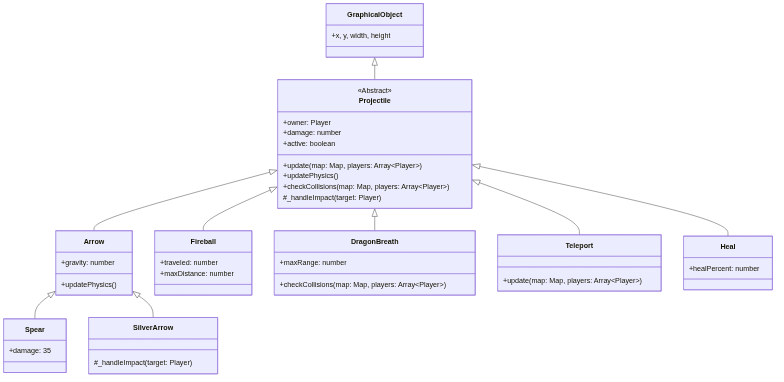
\includegraphics[width=1\textwidth]{canvas_3.png}
	\caption{Conception modulaire du système de balistique et des projectiles}
	\label{fig:projectiles}
\end{figure}
\FloatBarrier

Enfin, la véritable force de cette architecture réside dans l'utilisation de patrons de conception comportementaux éprouvés, notamment le patron Stratégie pour l'intelligence artificielle et le patron Commande pour le système de compétences. Plutôt que de coder en dur les prises de décision des ennemis dans leurs classes respectives, nous leur injectons dynamiquement une stratégie cognitive abstraite. Ainsi, un ennemi peut se voir assigner une intelligence basique se contentant de foncer en ligne droite, une intelligence avancée capable d'esquiver les obstacles et de prédire les chutes balistiques, ou encore une stratégie purement immobile. De manière analogue, toutes les actions des personnages sont encapsulées dans des classes de compétences indépendantes obéissant à une interface commune. Qu'il s'agisse de tirer une flèche physique, de lancer un sort de soin modifiant les statistiques internes, ou de se téléporter en manipulant les vecteurs spatiaux, chaque capacité gère de manière autonome son propre temps de recharge et son exécution. Ce paradigme rend l'ajout de nouvelles mécaniques de jeu extrêmement flexible, car les compétences sont totalement décorrélées de la logique interne des avatars qui les utilisent.

% ==========================================
% INSERTION DU DIAGRAMME 4 : PATRONS DE CONCEPTION
% Ce diagramme expose le pattern Strategy (AI) et Command (Abilities)
% ==========================================
\FloatBarrier
\begin{figure}[H]
	\centering
	% Remplacez 'patterns.png' par le nom exact de votre image exportée
	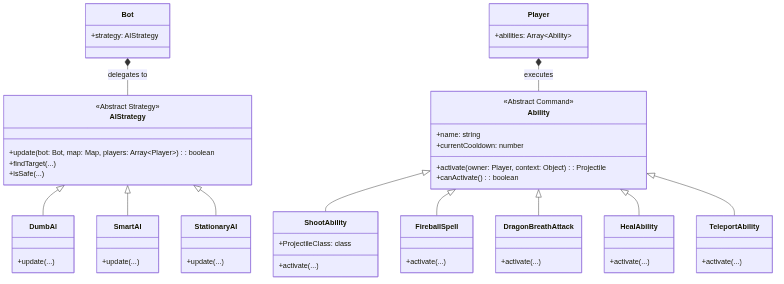
\includegraphics[width=1\textwidth]{canvas_4.png}
	\caption{Utilisation des patrons Stratégie (IA) et Commande (Compétences)}
	\label{fig:patterns}
\end{figure}
\FloatBarrier
	\section{Conception du Jeu DOM}

Le second jeu de notre suite, baptisé Dev Clicker, représente l'implémentation la plus simple de notre projet d'un point de vue architectural et algorithmique. Ce choix de conception minimaliste a été dicté en grande partie par des contraintes de temps, l'intégration complexe de BabylonJS et de WebAssembly ayant consommé la majorité de nos ressources de développement. Cependant, malgré cette simplicité apparente, le genre du jeu incrémental s'est avéré être le candidat absolument parfait pour démontrer notre maîtrise des mécanismes natifs du Document Object Model. En effet, un jeu de type clicker repose presque exclusivement sur la création d'éléments à la volée, la mise à jour massive de nœuds textuels en temps réel et l'écoute continue d'événements asynchrones, ce qui correspondait exactement aux exigences pédagogiques de cette partie de l'UE.

D'un point de vue technique, nous avons opté pour une architecture fonctionnelle basée sur des modules ES6, séparant de manière stricte la logique d'état, l'interface utilisateur et la gestion des entrées. Au cœur du système se trouve un objet d'état global faisant office de source de vérité unique pour toutes les métriques économiques, telles que les lignes de code générées, les multiplicateurs de rendement et les compteurs de cycles d'intelligence artificielle. Ce choix permet d'éviter l'éparpillement des données au sein des éléments HTML et garantit que la logique métier reste totalement découplée de la vue. La boucle principale du jeu interroge cet état à intervalles réguliers, agrège les rendements passifs de toutes les améliorations achetées, puis ordonne un rafraîchissement global des données à l'écran.

% ==========================================
% INSERTION DU DIAGRAMME : ARCHITECTURE DOM
% Ce diagramme montre l'interaction entre Main, GameState, UI et Events.
% ==========================================
\FloatBarrier
\begin{figure}[H]
	\centering
	% Remplacez 'dom_architecture.png' par le nom exact de votre image exportée
	
\includegraphics[width=1\textwidth]{dom.png}
	\caption{Architecture modulaire et flux de données du jeu DOM}
	\label{fig:dom_architecture}
\end{figure}
\FloatBarrier

Le gestionnaire d'interface agit comme le bras armé de l'application en manipulant directement l'arbre DOM. Au lancement du jeu, il lit un registre statique contenant la configuration de toutes les améliorations disponibles au magasin et génère dynamiquement les fragments HTML correspondants, les injectant ensuite dans le document de manière optimisée. De plus, il intègre un composant visuel original simulant un éditeur de code, dont le contenu se met à jour en repeignant sélectivement le DOM en fonction de l'accumulation historique des lignes de code du joueur. Les interactions de l'utilisateur avec ces éléments sont interceptées par un gestionnaire d'événements dédié, qui se charge de vérifier les conditions de ressources, de muter l'état global en conséquence, et d'ordonner une actualisation localisée de l'interface graphique pour refléter les nouveaux coûts.

Enfin, pour relier cette application purement client à notre écosystème global, un module de service dédié au score gère la fin de session. Ce service a pour rôle de créer et d'injecter une fenêtre modale de soumission directement dans le DOM, de figer la boucle de simulation pour empêcher toute triche de dernière minute, puis d'extraire la charge utile finale depuis le contenu textuel de l'éditeur virtuel. Cette valeur est ensuite encapsulée et expédiée vers notre interface de programmation applicative serveur sécurisée par un jeton d'authentification, bouclant ainsi l'expérience de manière fluide et persistante.
	\section{Conception du Jeu BabylonJS}

Le troisième et dernier jeu de notre suite est incontestablement le projet le plus ambitieux et le plus complexe sur le plan technique de notre rendu. L'objectif était de concevoir un jeu de stratégie hybride en trois dimensions, fusionnant les mécaniques économiques et de placement d'un \textit{Auto-Chess} (inspiré de \textit{Teamfight Tactics}) avec les règles de déplacement du jeu d'échecs traditionnel. Pour soutenir une telle architecture, nous avons abandonné les configurations classiques au profit de \textit{Vite}, un outil de construction moderne et ultra-rapide. L'utilisation de Vite s'est avérée indispensable pour gérer efficacement le remplacement de modules à chaud (HMR) durant le développement, tout en offrant un empaquetage hautement optimisé pour nos ressources volumineuses, nos modèles tridimensionnels et nos modules compilés.

% ==========================================
% INSERTION DU DIAGRAMME 1 : CŒUR & VITE
% ==========================================
\FloatBarrier
\begin{figure}[H]
	\centering
	% Remplacez par le nom de votre fichier exporté
	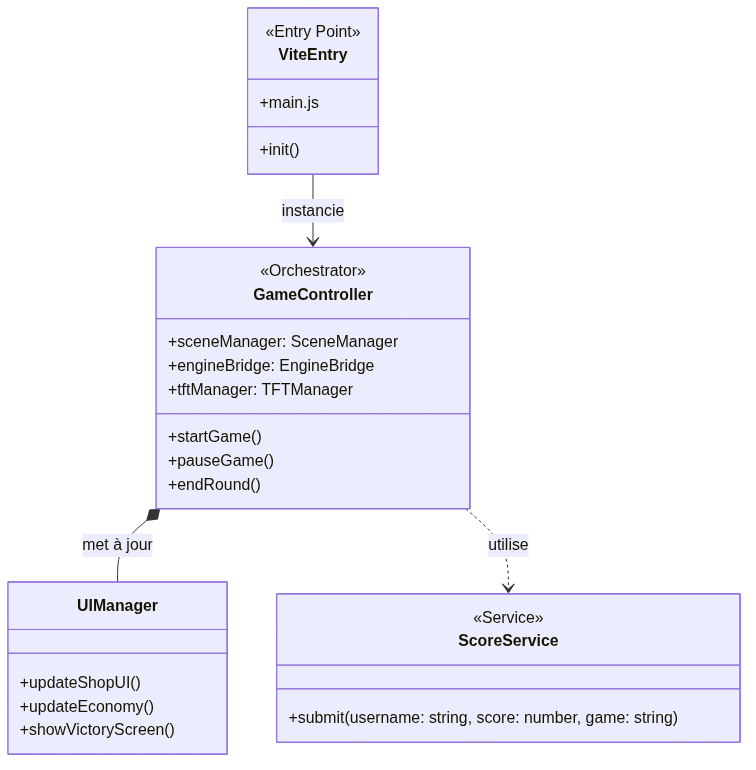
\includegraphics[width=0.8\textwidth]{babylon_1.png}
	\caption{Architecture principale et orchestration via l'environnement Vite}
	\label{fig:babylon_core}
\end{figure}
\FloatBarrier

La couche visuelle repose entièrement sur le framework BabylonJS, qui nous a permis de générer une scène tridimensionnelle performante exécutée directement dans le navigateur. La conception de cette couche est encapsulée dans un gestionnaire de scène dédié qui gère l'initialisation du moteur de rendu, le placement des caméras orbitales et le calcul de l'éclairage dynamique. Par-dessus cette scène, un chargeur de ressources asynchrone s'occupe de récupérer, de décoder et de mettre en cache nos modèles de pièces personnalisées au format GLB ou STL depuis le répertoire public. Les pièces sont ensuite liées à des objets logiques capables de transposer les coordonnées d'une grille d'échiquier mathématique abstraite vers des vecteurs spatiaux réels dans l'univers 3D, tout en gérant les animations de déplacement ou d'attaque.

% ==========================================
% INSERTION DU DIAGRAMME 2 : RENDU 3D
% ==========================================
\FloatBarrier
\begin{figure}[H]
	\centering
	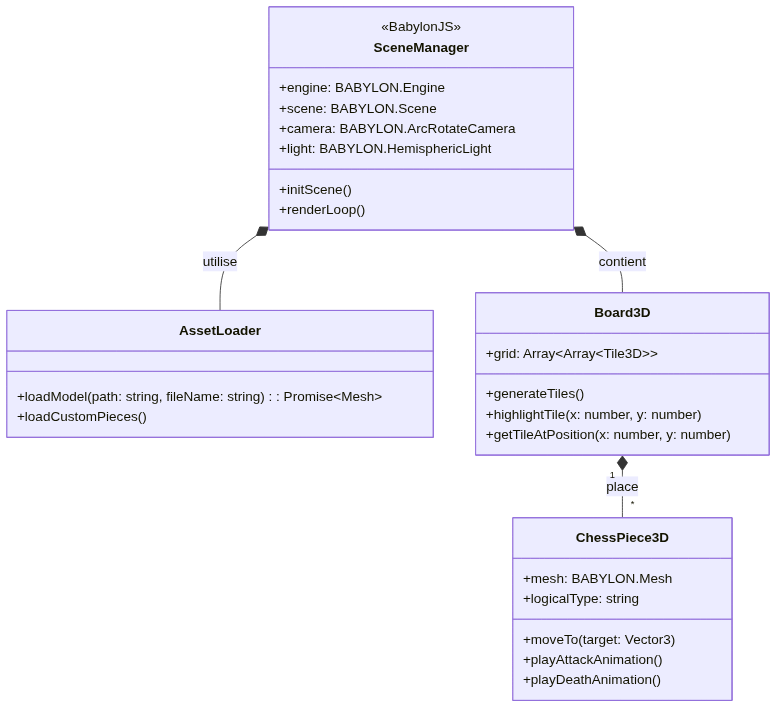
\includegraphics[width=0.8\textwidth]{babylon_2.png}
	\caption{Sous-système de rendu 3D et chargement asynchrone des modèles}
	\label{fig:babylon_3d}
\end{figure}
\FloatBarrier

La véritable complexité de ce projet réside toutefois dans son intelligence artificielle. Plutôt que de développer un algorithme d'échecs en JavaScript, ce qui aurait été bien trop lent, nous avons intégré \textit{Stockfish}, le moteur d'échecs open-source le plus puissant au monde. Pour ce faire, nous avons utilisé une version du moteur originellement écrit en C++, compilée en WebAssembly (WASM). Cette intégration a exigé la conception d'un pont de communication robuste. Le moteur WebAssembly s'exécute de manière isolée dans un \textit{Web Worker} afin de ne pas bloquer le fil d'exécution principal du navigateur gérant le rendu à soixante images par seconde. Le contrôleur du jeu traduit l'état actuel du plateau en notation Forsyth-Edwards (FEN), l'envoie au travailleur asynchrone, puis parse la réponse du moteur WASM pour animer les pièces adverses. Adapter ce moteur rigide à nos propres règles de pièces personnalisées et à notre plateau a constitué un défi architectural majeur.

% ==========================================
% INSERTION DU DIAGRAMME 3 : WEBASSEMBLY
% ==========================================
\FloatBarrier
\begin{figure}[H]
	\centering
	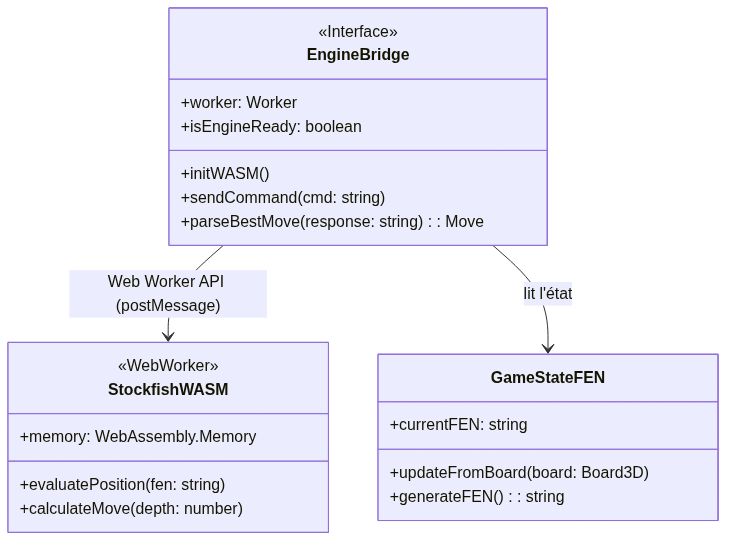
\includegraphics[width=0.8\textwidth]{babylon_3.png}
	\caption{Pont de communication asynchrone avec le moteur WebAssembly (Stockfish)}
	\label{fig:babylon_wasm}
\end{figure}
\FloatBarrier

Enfin, pour transformer ce simple jeu d'échecs en un véritable \textit{Auto-Chess}, nous avons implémenté une surcouche logique indépendante de la 3D et du moteur Stockfish. Cette couche est subdivisée en plusieurs gestionnaires spécialisés. Un gestionnaire d'économie calcule les revenus passifs, les intérêts et l'or généré par les séries de victoires ou de défaites. Un gestionnaire de boutique propose un choix aléatoire de pièces personnalisées à acheter entre chaque manche de combat. De plus, un gestionnaire de synergies analyse la composition de l'armée du joueur sur le plateau pour appliquer des modificateurs mathématiques globaux, affectant les calculs lors de la résolution du combat par WebAssembly. Cette stricte séparation des préoccupations permet au jeu de fonctionner par phases distinctes (draft et combat) sans créer de couplage fort entre l'interface utilisateur, la logique économique et les calculs du moteur.

% ==========================================
% INSERTION DU DIAGRAMME 4 : AUTO-CHESS LOGIC
% ==========================================
\FloatBarrier
\begin{figure}[H]
	\centering
	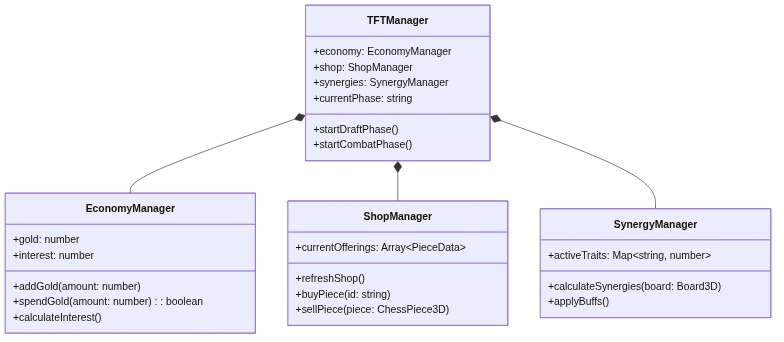
\includegraphics[width=0.8\textwidth]{babylon_4.png}
	\caption{Mécaniques Auto-Chess : Économie, Boutique et Synergies}
	\label{fig:babylon_tft}
\end{figure}
\FloatBarrier
	
\end{document}